\section{TỔNG QUAN}
\subsection{Bối cảnh phát triển}

Trong thời đại chuyển đổi số toàn diện, đặc biệt trong lĩnh vực y tế, việc áp dụng các công nghệ mới vào chăm sóc sức khỏe cá nhân ngày càng trở thành một nhu cầu cấp thiết. Tại Việt Nam, chính phủ đã ban hành nhiều chính sách nhằm thúc đẩy quá trình chuyển đổi số, trong đó y tế số là một trong những trọng điểm để cải thiện chất lượng chăm sóc và quản lý sức khỏe cộng đồng. Nhu cầu chăm sóc sức khỏe không chỉ dừng lại ở việc điều trị bệnh, mà còn mở rộng ra các hoạt động dự phòng và theo dõi liên tục tình trạng sức khỏe của cá nhân thông qua các thiết bị điện tử thông minh. 

Sự phát triển của các thiết bị y tế thông minh, đặc biệt là những thiết bị gắn liền với Internet vạn vật (IoT), đã thay đổi cách người dùng tiếp cận việc chăm sóc sức khỏe. Thay vì phải dựa vào các cơ sở y tế và gặp gỡ bác sĩ thường xuyên, người dùng có thể tự theo dõi sức khỏe của mình ngay tại nhà một cách chính xác và liên tục. Điều này đặc biệt hữu ích trong việc phát hiện sớm các vấn đề sức khỏe, điều chỉnh lối sống, cũng như quản lý các bệnh mãn tính.

\subsection{Nhu cầu về chuyển đổi số trong lĩnh vực y tế tại Việt Nam \cite{cds1} \cite{cds2} \cite{cds3}}
Y tế số, còn được gọi là "Digital Health," là một lĩnh vực sử dụng công nghệ số hóa để cải thiện việc quản lý sức khỏe, chẩn đoán, điều trị và dịch vụ y tế. Lĩnh vực này kết hợp các công nghệ hiện đại như thông tin, ứng dụng di động, cảm biến, trí tuệ nhân tạo và học máy. Các công nghệ ứng dụng trong y tế số đã giúp thúc đẩy chuyển đổi số trong lĩnh vực y tế. Một số công cụ và ứng dụng hiện đại đã được sử dụng để cải thiện y tế số có thể kế đến như:

\begin{itemize}
    \item \textbf{Hồ sơ y tế điện tử} là một hệ thống cho phép lưu trữ và quản lý thông tin y tế của bệnh nhân một cách điện tử, giúp tăng tính hiệu quả và giảm sai sót trong quản lý hồ sơ bệnh nhân.
    \item \textbf{Telehealth và Telemedicine} là phương pháp khám bệnh từ xa thông qua video cuộc gọi, điện thoại và ứng dụng di động, giúp bệnh nhân tiếp cận dịch vụ y tế một cách dễ dàng và thuận tiện.
    \item \textbf{Internet of Things (IoT)} trong y tế liên kết các thiết bị y tế với internet để thu thập dữ liệu sức khỏe của bệnh nhân, giúp theo dõi và quản lý sức khỏe cá nhân một cách hiệu quả.
    \item \textbf{Máy học (Machine Learning) và Trí tuệ nhân tạo (AI)} được ứng dụng trong y tế để phân tích dữ liệu y tế phức tạp, hỗ trợ chẩn đoán, dự đoán xu hướng dịch bệnh và tạo ra giải pháp điều trị cá nhân hóa.
    \item \textbf{Ứng dụng di động y tế} cho phép bệnh nhân quản lý sức khỏe, đặt lịch hẹn và nhận thông tin về dược phẩm hoặc hẹn tái khám một cách dễ dàng và tiện lợi.
    \item \textbf{Công nghệ Blockchain trong Y tế} được sử dụng để bảo vệ thông tin y tế và đảm bảo tính bảo mật trong việc chia sẻ dữ liệu bệnh nhân.
\end{itemize}

\subsubsection{Những đóng góp của chuyển đổi số với ngành y tế}
\textbf{Đối với người dân:}

Chuyển đổi số y tế tạo cơ hội để người dân dễ dàng tiếp cận các dịch vụ chăm sóc sức khỏe, tương tác với nhân viên y tế và quản lý sức khỏe cá nhân thông qua kết nối dữ liệu sức khỏe với các cơ sở khám chữa bệnh. Mục tiêu cuối cùng là đảm bảo mỗi người dân sở hữu hồ sơ sức khỏe điện tử. Việc áp dụng công nghệ 4.0 trong chuyển đổi số y tế giúp cải thiện tính cá nhân hóa trong chăm sóc sức khỏe và cứu sống bệnh nhân trong các trường hợp khẩn cấp.

Đặc biệt, các công nghệ mới như hồ sơ điện tử và hệ thống thông tin y tế liên kết giúp tăng cường khả năng chia sẻ thông tin y tế giữa các cơ sở chăm sóc. Điều này cung cấp thông tin quan trọng, chính xác cho việc chẩn đoán và điều trị, giúp nâng cao chất lượng dịch vụ y tế.

\begin{figure}[!htp]
    \centering
    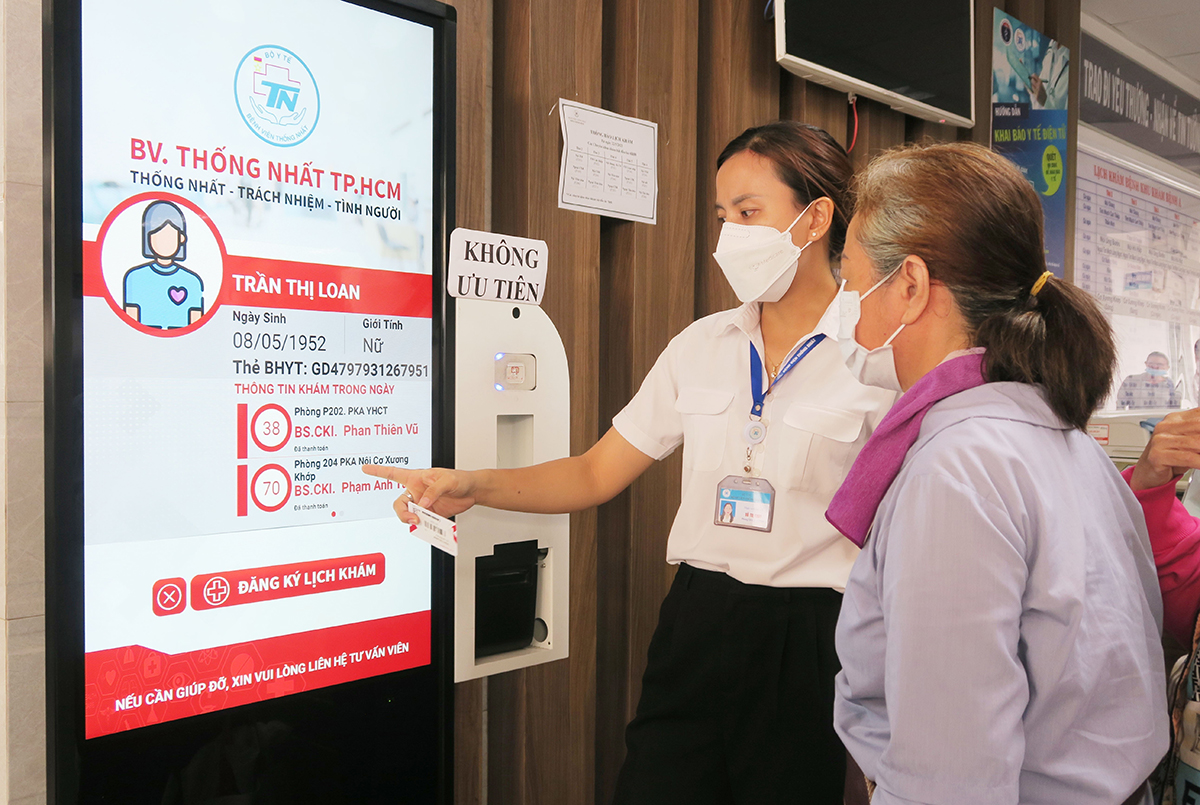
\includegraphics[width=0.5\linewidth]{graphics/ngdan_yte.png}
    \caption{Người bệnh đăng ký khám bệnh tại bảng thông tin điện tử của Bệnh viện Thống Nhất Thành phố Hồ Chí Minh\_Ảnh: TTXVN}
\end{figure}

\textbf{Đối với nhân viên y tế:}

Chuyển đổi số y tế giúp các bác sĩ dễ dàng tiếp cận kiến thức và kỹ thuật y học mới nhất, nâng cao chất lượng và an toàn cho bệnh nhân. Ngoài ra, chuyển đổi số cũng giảm thiểu nguy cơ sai sót trong các quy trình y tế, đảm bảo sự chính xác và đáng tin cậy trong quản lý thông tin y tế. Các công nghệ mới giúp nhân viên y tế cải thiện hiệu suất và chất lượng công việc, đồng thời nâng cao sự hài lòng của bệnh nhân.
Hệ thống quản lý thông tin y tế đã giúp tạo điều kiện thuận lợi cho việc truy cập và chia sẻ thông tin của bệnh nhân giữa các bác sĩ, cơ sở khám chữa bệnh. Điều này cho phép các chuyên gia y tế kết nối và tương tác dễ dàng hơn.

Mục tiêu của việc chuyển đổi số y tế là xây dựng hồ sơ bệnh án điện tử tại mỗi bệnh viện và cơ sở khám chữa bệnh.

Chuyển đổi số trong lĩnh vực y tế mang lại nhiều lợi ích cho việc quản lý sức khỏe và cung cấp dịch vụ chăm sóc. Công nghệ giúp các nhà quản lý y tế hiệu quả hơn trong công tác điều phối, giám sát, cảnh báo và dự báo về các vấn đề sức khỏe của người dân.
Chuyển đổi số đóng vai trò hết sức quan trọng trong tiến trình cải cách thủ tục hành chính của ngành y tế. Bằng việc áp dụng các ứng dụng và hệ thống trực tuyến, ngành y tế có thể giảm thiểu các thủ tục phức tạp, thời gian chờ đợi và cung cấp dịch vụ chăm sóc sức khỏe thuận lợi hơn cho người dân.

Chuyển đổi số cũng giúp tăng cường tính tiếp cận và hiệu quả khi thực hiện các dịch vụ y tế. Từ đó, chất lượng phục vụ cho người bệnh và nhân viên y tế có thể được nâng cao đáng kể.

Các ứng dụng hữu ích của chuyển đổi số cũng mang lại nhiều lợi ích cho nhà quản lý bệnh viện và cơ sở y tế. Các ứng dụng này giúp quản lý quy trình, phác đồ điều trị của nhân viên y tế và triển khai các công việc nhằm nâng cao chất lượng phục vụ cho người bệnh và nhân viên y tế.

\newpage

\begin{figure}[!htp]
    \centering
    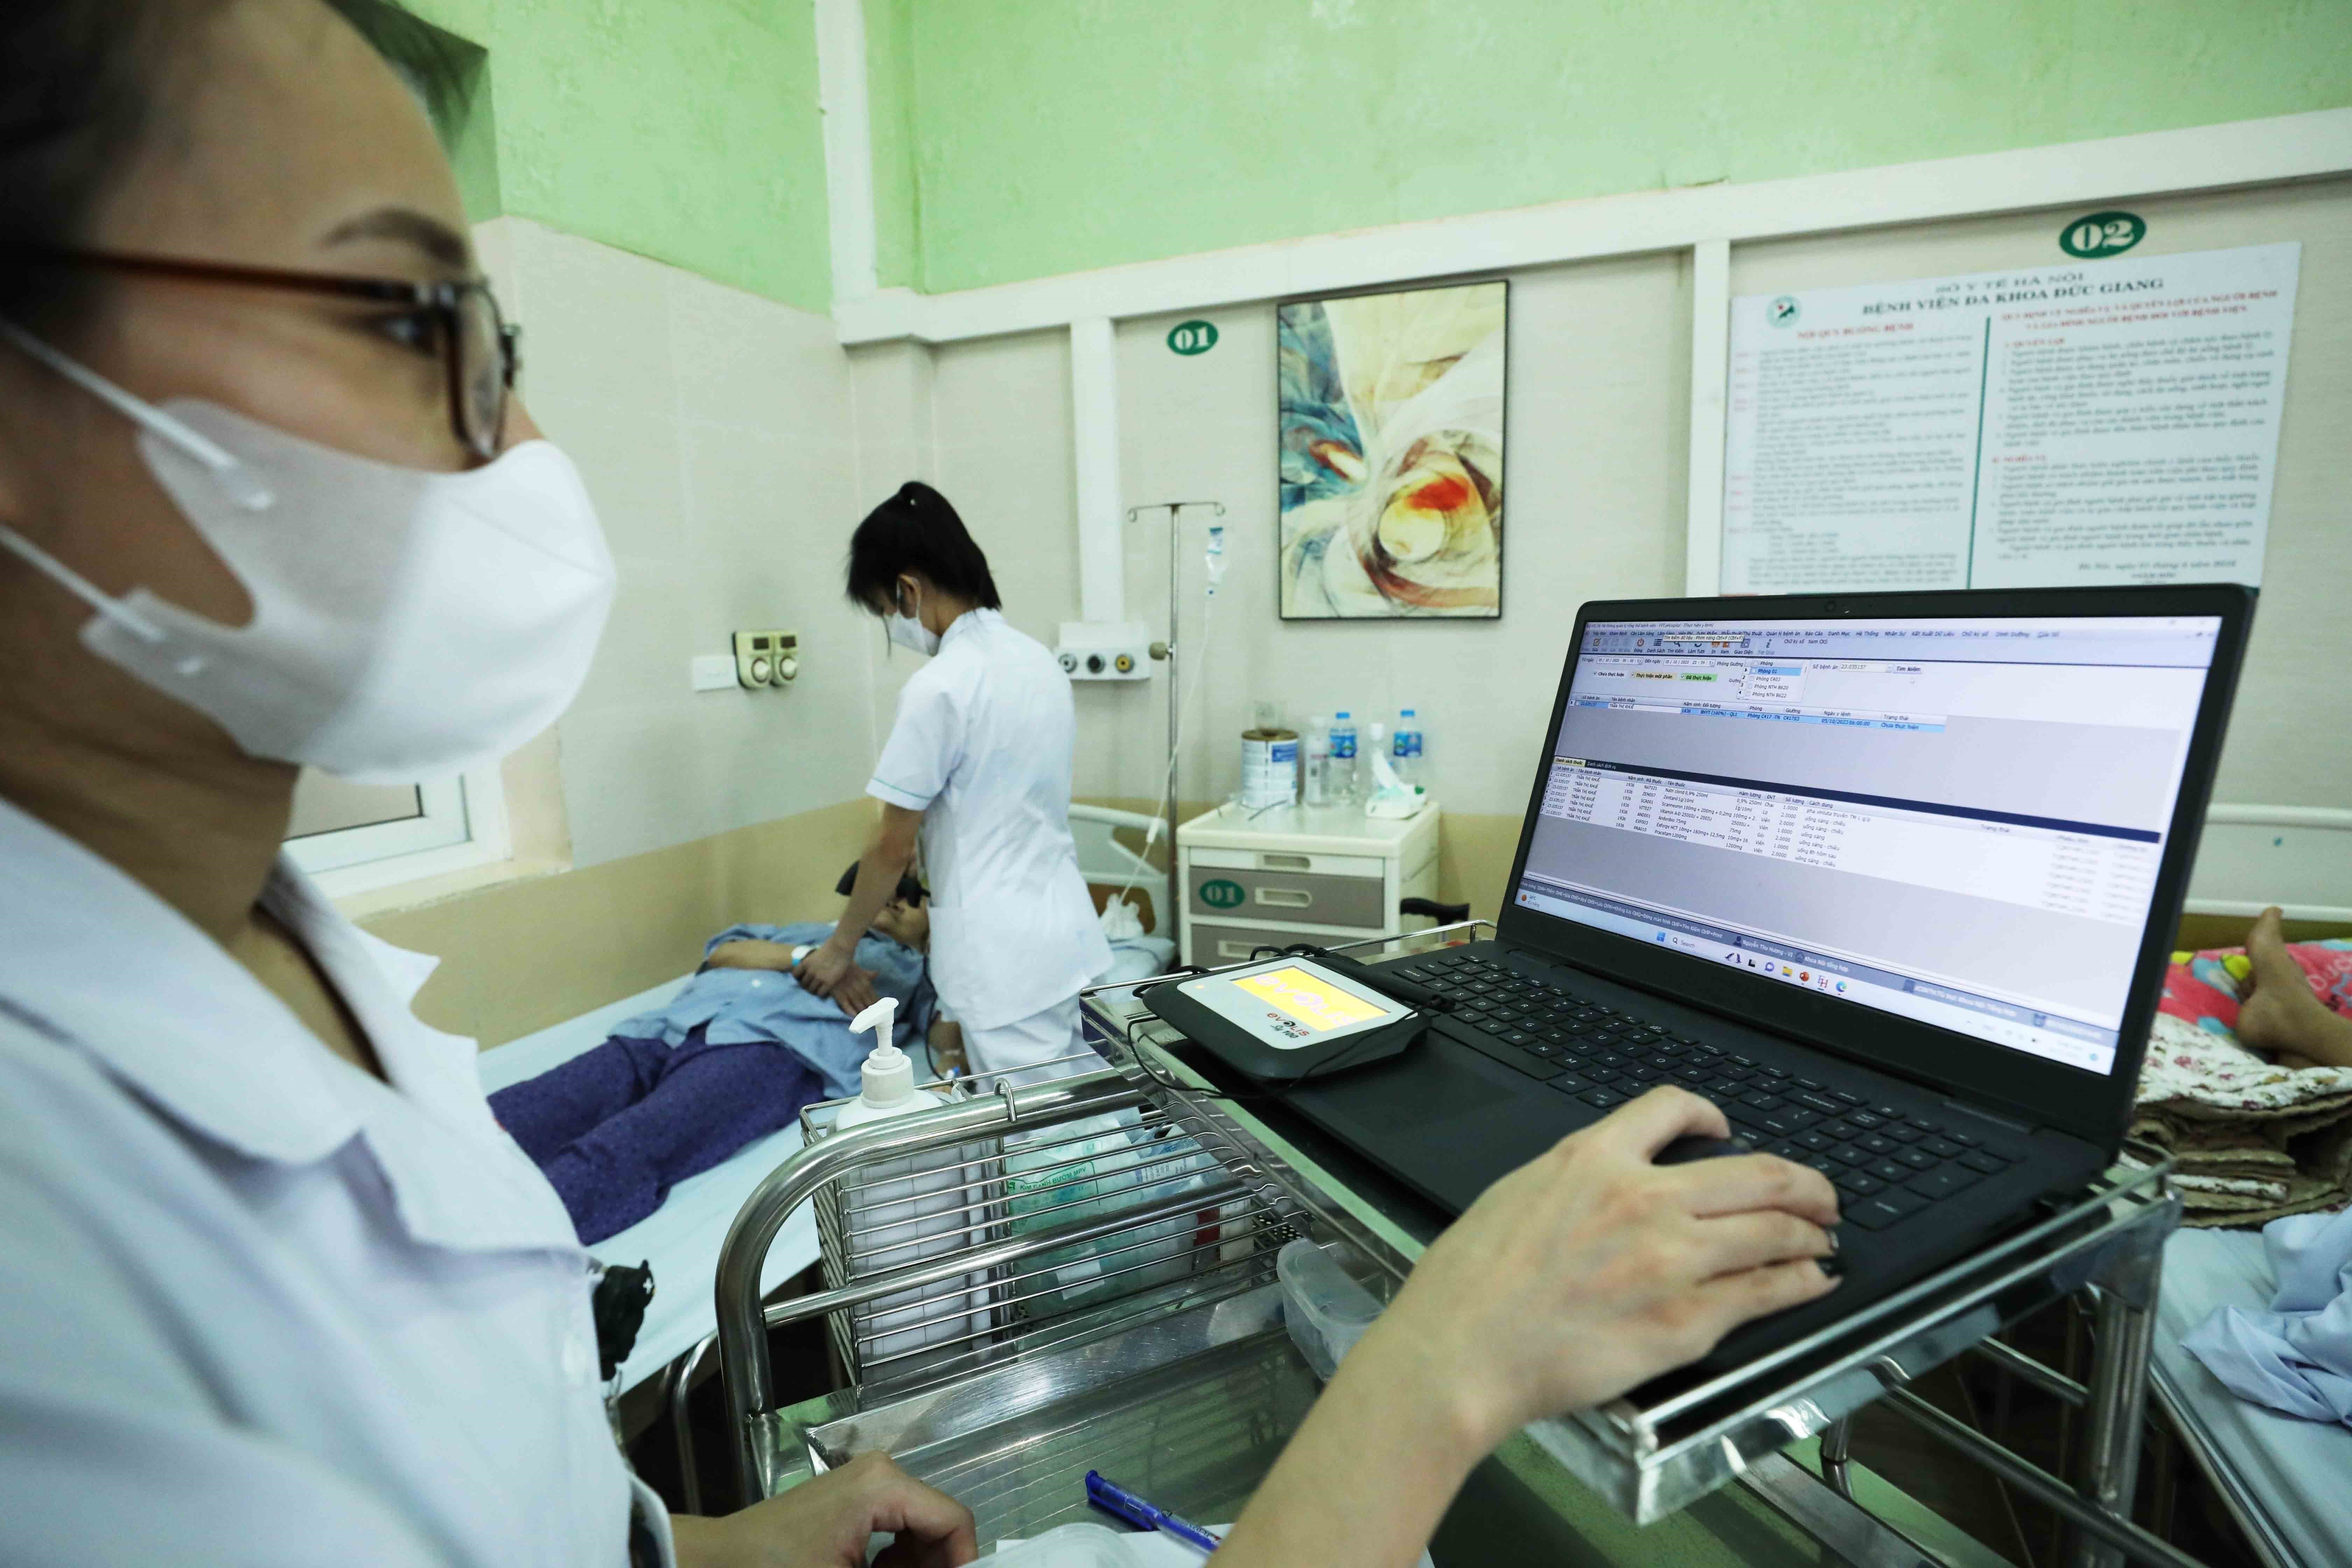
\includegraphics[width=0.6\linewidth]{graphics/bacsi_qr.png}
    \caption{Bệnh viện Đa khoa Đức Giang sử dụng mã QR Code cấp cho bệnh nhân giúp điều dưỡng viên nắm thông tin bệnh nhân thông qua thiết bị quét mã, hiển thị lên màn hình máy tính đặt trên xe thuốc\_Ảnh: TTXVN}
\end{figure}

\subsubsection{Thực trạng chuyển đổi số y tế tại Việt Nam}
Một nghiên cứu gần đây của Trường Đại học Kinh tế Tp. Hồ Chí Minh đã chỉ ra rằng Việt Nam, đặc biệt là TP.HCM, đã tương đối kiểm soát và ổn định được tình hình đại dịch COVID-19 trong vài năm trở lại đây. Dù đã kiểm soát được đại dịch nhưng dấu ấn còn lại của sự tàn phá khủng khiếp vẫn tiếp tục đọng lại trong tâm trí người dân.

Trong bối cảnh ứng dụng Công nghệ thông tin và chuyển đổi số trong công tác phòng chống dịch, Thành phố Hồ Chí Minh đã thể hiện sự sáng tạo và hiệu quả đáng ghi nhận. Một ví dụ điển hình cho điều này là hệ thống quản lý người bệnh COVID-19 được Sở Y tế TP.HCM phát triển và ra mắt vào đầu tháng 3/2022.

Trước đó, hàng nghìn người đến các trung tâm y tế chờ đợi để khai báo đã mắc COVID-19 (F0) và hàng nghìn người khác chờ đợi để nhận giấy xác nhận đã hoàn thành thời gian cách ly tại nhà. Tuy nhiên, nhờ vào hệ thống quản lý này, Thành phố đã giải quyết triệt để tình trạng tắc nghẽn của người bệnh tại các trung tâm y tế trên toàn thành phố.
Việt Nam đang đặt phát triển chăm sóc sức khỏe là một ưu tiên hàng đầu. Chi tiêu cho lĩnh vực y tế đang có sự tăng trưởng mạnh mẽ, từ 15,6 tỷ USD trong năm 2018 lên 42,9 tỷ USD vào năm 2028, tương đương mức tăng trưởng kép hàng năm (CAGR) là 11\% trong 10 năm. Điều này giúp Việt Nam trở thành quốc gia đầu tư nhiều nhất vào lĩnh vực chăm sóc sức khỏe trong khu vực ASEAN. Mức chi tiêu bình quân đầu người cho chăm sóc sức khỏe cũng dự kiến sẽ tăng lên 408 USD/năm vào năm 2028, gấp ba lần so với mức 141 USD/năm năm 2018.

Việt Nam có nhiều điều kiện thuận lợi để áp dụng các giải pháp y tế số. Các công nghệ mới đã nhanh chóng được đón nhận bởi hơn 60\% dân số Việt Nam dưới 54 tuổi. Người dân Việt Nam dành khoảng 7 giờ mỗi ngày cho các hoạt động trực tuyến, và 3 giờ trong số đó được thực hiện trên các thiết bị di động.

Việt Nam đã thực hiện nhiều chính sách để xây dựng cơ sở hạ tầng và phát triển các dịch vụ công nghệ thông tin và truyền thông. Việc truy cập internet đã được lan rộng trên toàn quốc, với tỷ lệ sử dụng đạt 67\% vào năm 2017, và tốc độ tăng trưởng hàng năm của việc sử dụng internet là 28\%. Công nghệ thông tin di động cũng đang phát triển mạnh mẽ tại Việt Nam, với mạng 4G đã có phủ sóng đến hơn 95\% các hộ gia đình.

Việc áp dụng các giải pháp y tế số tại Việt Nam sẽ mang lại nhiều lợi ích. Điều này bao gồm khả năng truy cập thông tin y tế và dịch vụ y tế từ xa, cũng như khả năng theo dõi và quản lý sức khỏe của người dân một cách hiệu quả hơn.

Cơ sở hạ tầng công nghệ ở Việt Nam đang hướng tới việc ứng dụng các dịch vụ dựa trên nền tảng lưu trữ đám mây, tạo điều kiện thuận lợi cho việc triển khai các giải pháp sáng tạo và hiệu quả về chi phí trong lĩnh vực chăm sóc sức khỏe.

Bộ Y tế đã đưa ra một kế hoạch để triển khai ứng dụng công nghệ thông tin và chuyển đổi số tại các cơ sở khám chữa bệnh. Theo đó, các bệnh viện sẽ phải thực hiện chuyển đổi số trước ngày 1/1/2027 để được cấp giấy phép hoạt động kể từ năm nay.

Các bệnh viện được cấp giấy phép hoạt động trước ngày 1/1/2027 sẽ có thời gian đến ngày 1/1/2029 để hoàn thành chuyển đổi số.

\begin{figure}[!htp]
    \centering
    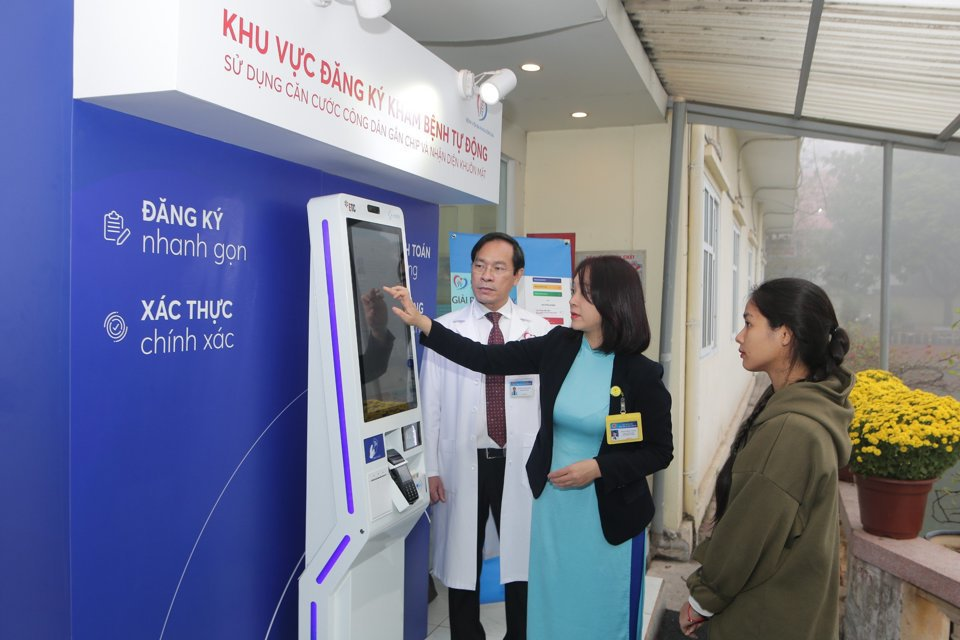
\includegraphics[width=0.6\linewidth]{graphics/faceid.png}
    \caption{Bệnh viện Đa khoa Đống Đa đã lắp đặt tại sảnh khoa Khám bệnh một máy đăng ký khám bệnh và phát số tự động sử dụng CCCD gắn chíp và nhận diện khuôn mặt.}
\end{figure}

\subsection{Thiết bị cân điện tử thông minh và tiềm năng ứng dụng}

Thị trường cân sức khỏe thông minh hiện nay đang ngày càng đa dạng với nhiều lựa chọn hấp dẫn như \textbf{Xiaomi Smart Scale 2} và \textbf{CRENOT Gofit S2}. Cả hai thiết bị này đều được trang bị công nghệ hiện đại, giúp người dùng theo dõi sức khỏe một cách chính xác và tiện lợi.

\textbf{Xiaomi Smart Scale 2} nổi bật với thiết kế đơn giản, hiện đại và khả năng kết nối nhanh chóng với ứng dụng Mi Fit. Thiết bị này cho phép người dùng đo được nhiều chỉ số cơ thể quan trọng như cân nặng, chỉ số khối cơ thể (BMI), tỷ lệ mỡ trong cơ thể, lượng nước trong cơ thể và khối lượng xương. Bên cạnh đó, Xiaomi Smart Scale 2 còn có khả năng nhận diện tới 16 người dùng khác nhau, rất phù hợp với những gia đình đông thành viên.

\begin{figure}[!htp]
    \centering
    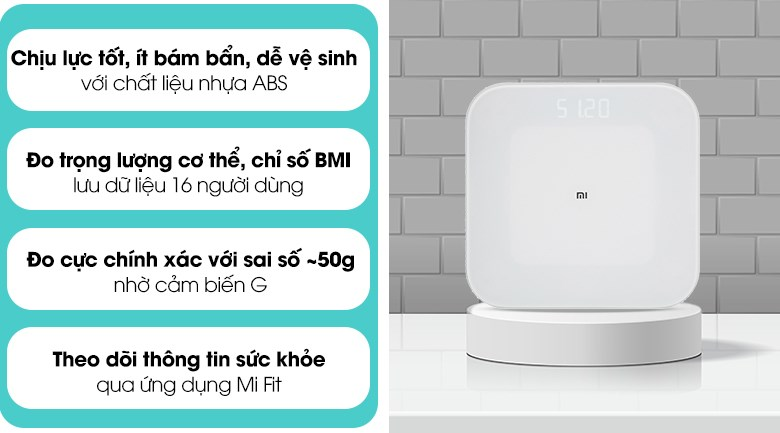
\includegraphics[width=0.8\linewidth]{graphics/xiaomi_scale2.jpg}
    \caption{Thông tin chi tiết của sản phẩm Xiaomi Smart Scale 2}
\end{figure}

Trong khi đó, \textbf{CRENOT Gofit S2} lại gây ấn tượng với độ chính xác cao nhờ sử dụng công nghệ phân tích trở kháng điện sinh học (BIA) kết hợp với chip cảm biến ZeroVar. Thiết bị này cung cấp một danh sách dài các chỉ số sức khỏe chi tiết hơn, giúp người dùng có cái nhìn toàn diện về tình trạng cơ thể của mình. Ngoài ra, CRENOT Gofit S2 còn có khả năng đồng bộ dữ liệu với nhiều ứng dụng sức khỏe khác nhau, tạo điều kiện cho người dùng quản lý thông tin một cách linh hoạt.

\newpage

\begin{figure}[!htp]
    \centering
    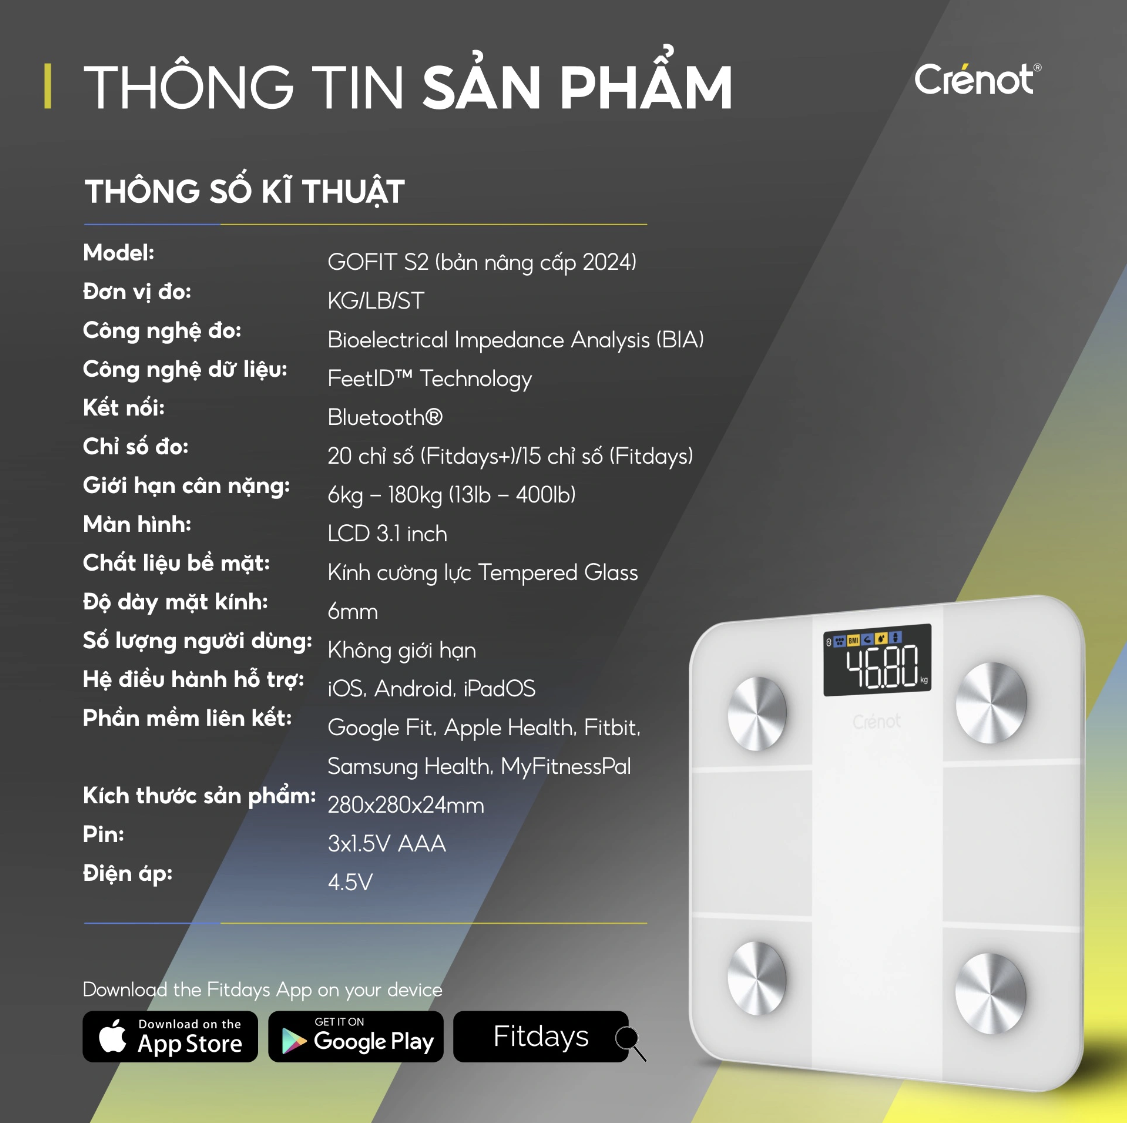
\includegraphics[width=0.7\linewidth]{graphics/info_crenot.png}
    \caption{Thông tin chi tiết của sản phẩm CRENOT Gofit S2}
\end{figure}

Xây dựng hệ thống chăm sóc sức khỏe điện tử với thiết bị cân điện tử sức khoẻ thông minh không chỉ mang lại những lợi ích cho cá nhân người sử dụng, mà còn đóng góp vào quá trình quản lý sức khỏe cộng đồng tại Việt Nam. Hệ thống này sẽ tận dụng dữ liệu được thu thập từ các thiết bị để cung cấp thông tin tổng quan về sức khỏe, giúp người dùng để phát hiện sớm những thay đổi tiêu cực trong cơ thể và có các biện pháp can thiệp kịp thời. 

Ngoài ra, hệ thống còn có thể tích hợp với các nền tảng khác như điện thoại thông minh, máy tính bảng và máy tính cá nhân thông qua các ứng dụng y tế hoặc nền tảng quản lý sức khỏe từ xa. Dữ liệu từ thiết bị cân thông minh được truyền qua kết nối Bluetooth hoặc Wi-Fi đến các ứng dụng quản lý sức khỏe, từ đó được lưu trữ trên hệ thống đám mây. Nhờ vào việc sử dụng trí tuệ nhân tạo (AI) và các công cụ phân tích dữ liệu lớn (Big Data), hệ thống có khả năng phân tích, đưa ra các gợi ý về sức khỏe, từ khuyến nghị về chế độ ăn uống, tập luyện cho đến các cảnh báo về nguy cơ bệnh tật.

Với xu hướng chuyển đổi số tại Việt Nam, hệ thống này còn có tiềm năng tích hợp với các hệ thống quản lý y tế cộng đồng, giúp các cơ sở y tế và bệnh viện dễ dàng theo dõi sức khỏe từ xa của bệnh nhân, đặc biệt là các bệnh nhân mắc bệnh mãn tính như tiểu đường, huyết áp cao hay béo phì. Điều này sẽ giảm tải áp lực cho hệ thống y tế, đặc biệt trong bối cảnh bệnh viện và các cơ sở y tế đang quá tải do số lượng bệnh nhân lớn.

\subsection{Các hệ thống tham chiếu trong nghiên cứu}
\subsubsection{Cân thông minh Xiaomi Body Scale S400 \cite{s400:online}}
Xiaomi Body Scale S400 là sản phẩm được người tiêu dùng sử dụng rộng rãi và vô cùng phổ biến ở thị trường trong và ngoài nước cũng là một trong những thiết bị thông minh đáng chú ý trong hệ sinh thái Xiaomi, được thiết kế để trở thành thiết bị chăm sóc sức khoẻ đáng tin cậy cho mỗi thành viên trong gia đình. Với thiết kế hiện đại và khả năng đo lường chính xác, sản phẩm này mang đến cho người dùng cái nhìn sâu sắc về tình trạng sức khỏe của bản thân, từ đó hỗ trợ xây dựng một lối sống lành mạnh và bền vững.

\begin{figure}[!htp]
    \centering
    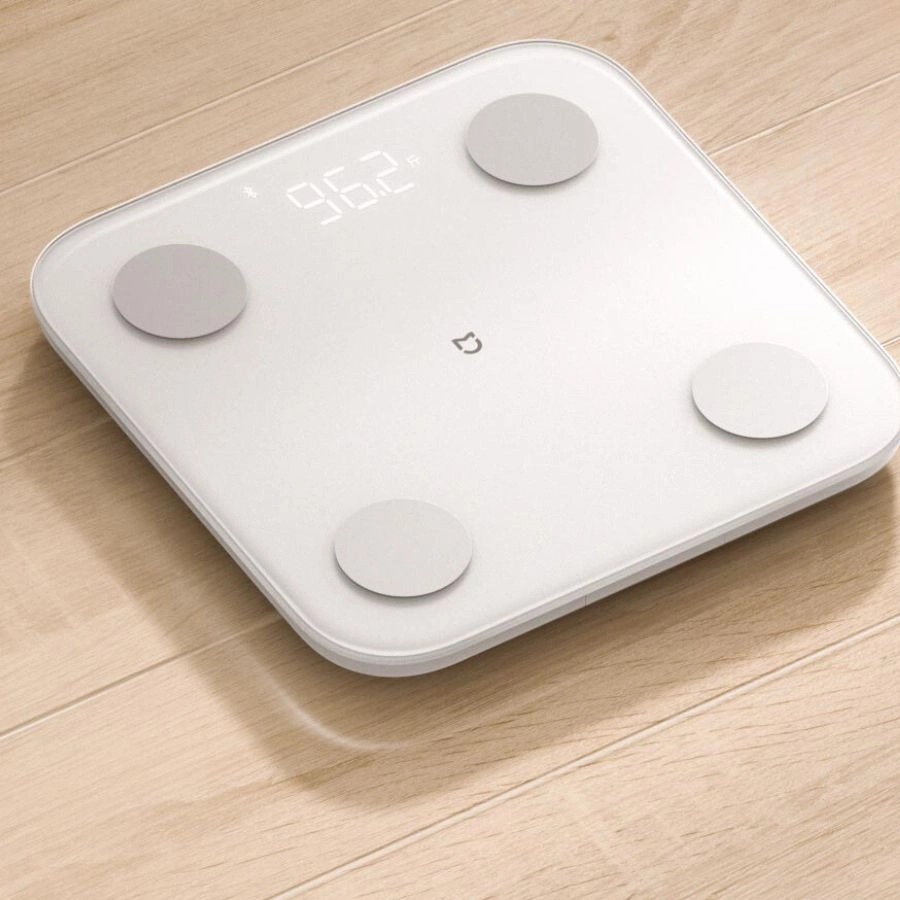
\includegraphics[width=0.6\linewidth]{graphics/s400.png}
    \caption{Cân Thông Minh Xiaomi Body Scale S400}
\end{figure}

Không chỉ đơn thuần là một chiếc cân, Xiaomi Body Scale S400 còn là một công cụ phân tích cơ thể toàn diện. Thiết bị này cung cấp hơn 10 chỉ số sức khỏe quan trọng, bao gồm một số tính năng nổi bật như:

\begin{itemize}
    \item \textbf{Cân nặng:} Theo dõi sự thay đổi cân nặng theo thời gian để đánh giá hiệu quả của quá trình giảm cân hoặc tăng cân.
    \item \textbf{Chỉ số khối cơ thể (BMI):} Đánh giá tình trạng cân nặng có phù hợp với chiều cao hay không, từ đó xác định nguy cơ mắc các bệnh liên quan đến béo phì hoặc suy dinh dưỡng.
    \item \textbf{Tỷ lệ mỡ cơ thể:} Cho biết lượng mỡ trong cơ thể, giúp bạn điều chỉnh chế độ ăn uống và tập luyện để đạt được tỷ lệ mỡ lý tưởng.
    \item \textbf{Tỷ lệ cơ bắp:} Đánh giá khối lượng cơ, giúp bạn theo dõi sự phát triển cơ bắp và xây dựng cơ thể săn chắc.
    \item \textbf{Khối lượng xương:} Giúp bạn theo dõi sức khỏe xương và phòng ngừa các bệnh về xương khớp.
    \item \textbf{Tỷ lệ nước trong cơ thể:} Cho biết lượng nước trong cơ thể, giúp bạn điều chỉnh lượng nước uống hàng ngày để duy trì sự cân bằng điện giải.
    \item Và nhiều chỉ số khác: Như khối lượng nội tạng, tuổi cơ thể, v.v., giúp bạn hiểu rõ hơn về tình trạng sức khỏe của mình.
\end{itemize}

\begin{figure}[!htp]
    \centering
    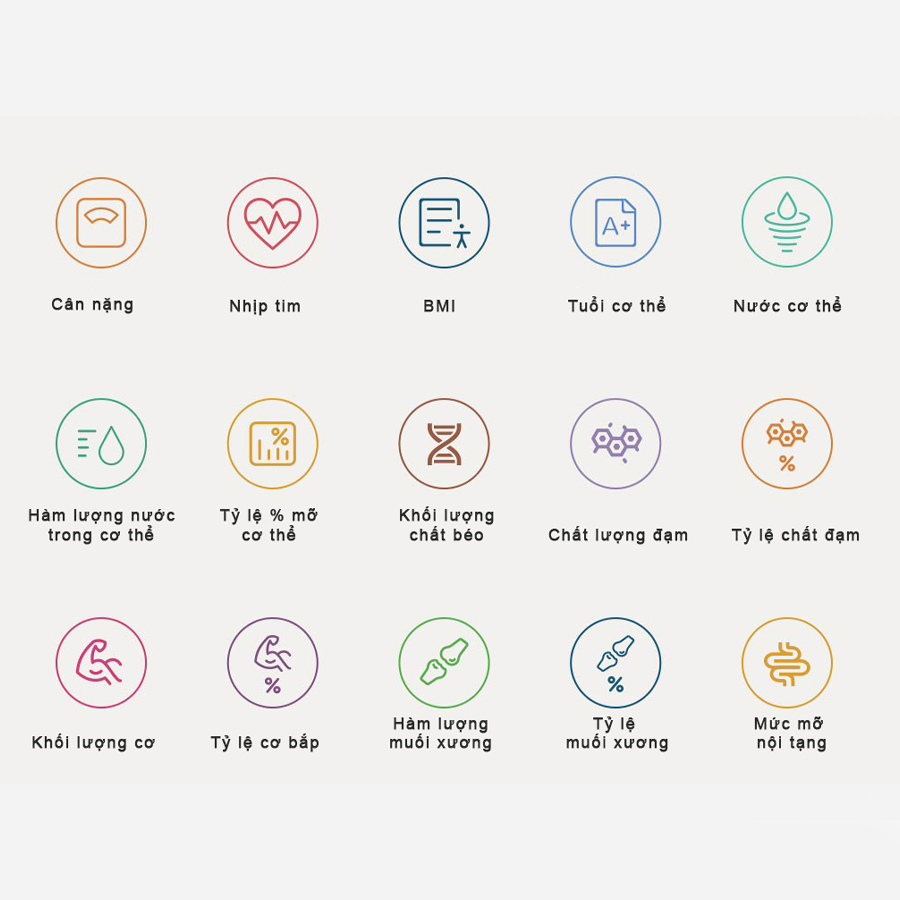
\includegraphics[width=0.6\linewidth]{graphics/thong_so_sk.png}
    \caption{Sự đa dạng về các chỉ số sức khoẻ mà S400 có thể đo được}
\end{figure}

Cân thông minh Xiaomi Body Scale S400 có thể kết nối với ứng dụng Mi Fit hoặc Zepp Life thông qua Bluetooth. Nhờ đó, người dùng có thể:

\begin{itemize}
    \item \textbf{Theo dõi dữ liệu theo thời gian thực:} Quan sát sự thay đổi của các chỉ số sức khỏe qua từng ngày, tuần hoặc tháng.
    \item \textbf{Trực quan hóa kết quả:} Biểu đồ và đồ thị trực quan giúp bạn dễ dàng nắm bắt tình hình sức khỏe của mình.
    \item \textbf{Nhận khuyến nghị cá nhân hóa:} Ứng dụng sẽ đưa ra các gợi ý về chế độ ăn uống và tập luyện phù hợp với mục tiêu của bạn.
    \item \textbf{Chia sẻ dữ liệu với chuyên gia:} Bạn có thể chia sẻ dữ liệu với bác sĩ hoặc chuyên gia dinh dưỡng để được tư vấn cụ thể hơn.
\end{itemize}

\begin{figure}[!htp]
    \centering
    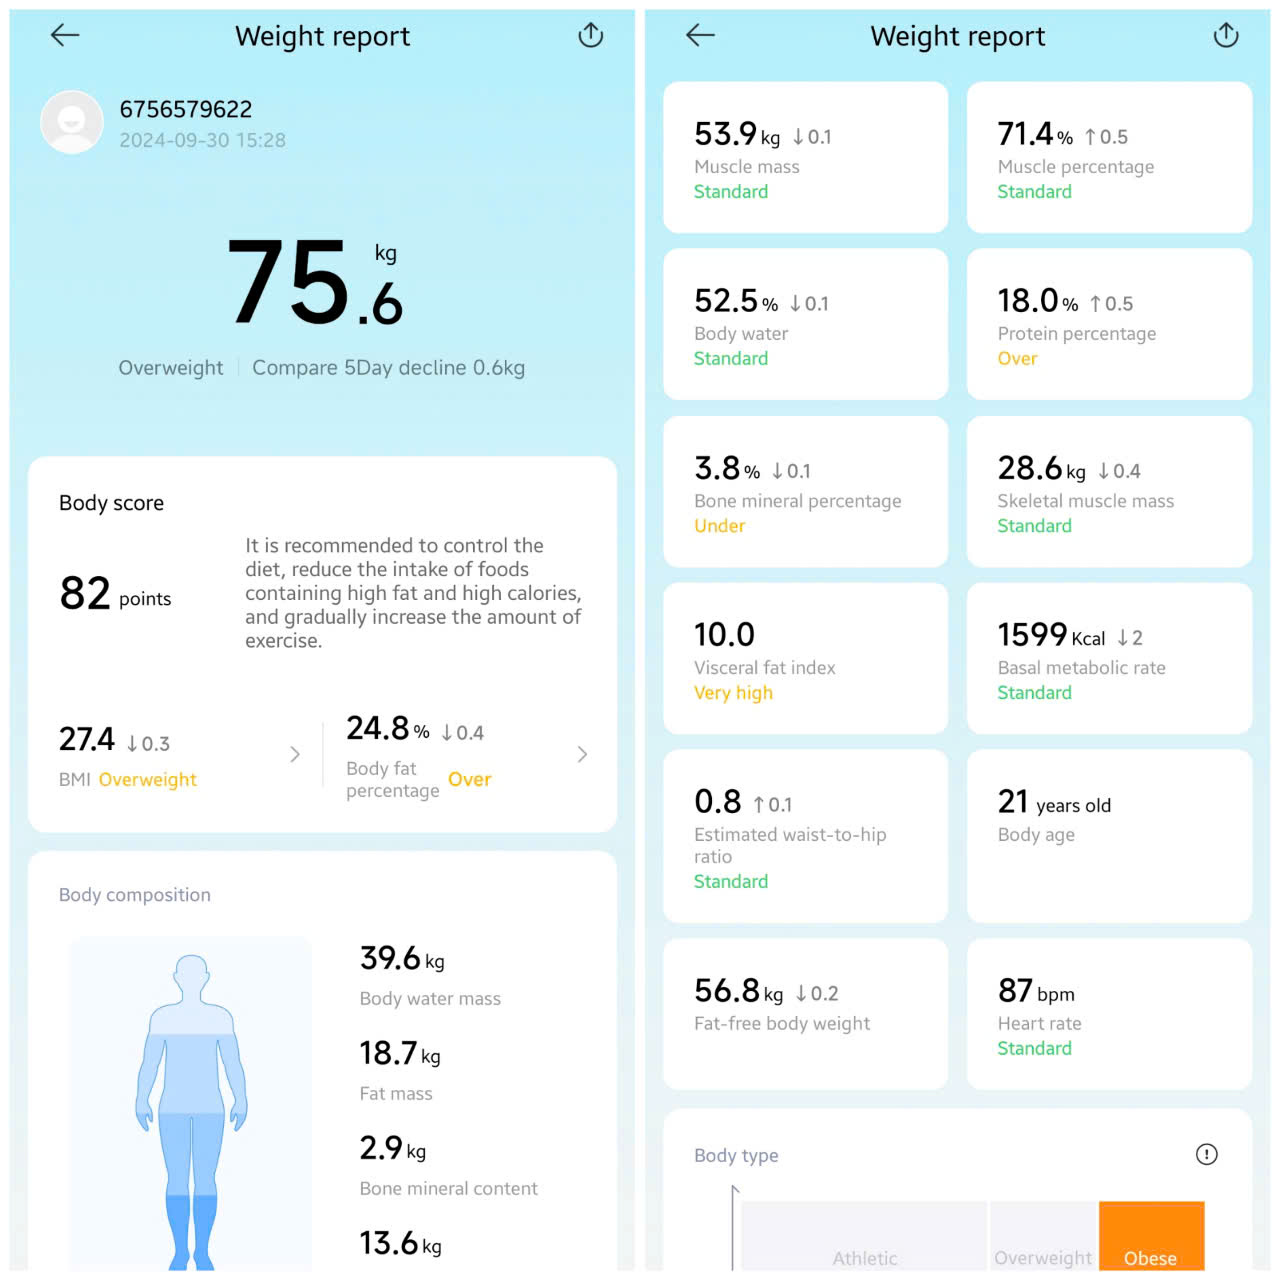
\includegraphics[width=0.5\linewidth]{graphics/info_user.png}
    \caption{Các chỉ số sức khoẻ của người dùng được thể hiện và đồng bộ hoá trên ứng dụng Mi Home}
\end{figure}

Xiaomi Body Scale S400 là một phần không thể thiếu trong hệ sinh thái nhà thông minh của Xiaomi. Người dùng có thể kết nối cân với các thiết bị khác như đồng hồ thông minh, điện thoại di động để tạo ra một hệ thống quản lý sức khỏe toàn diện.

\textbf{Ưu điểm nổi bật:}
\begin{itemize}
    \item \textbf{Thiết kế hiện đại, sang trọng:} Phù hợp với mọi không gian sống.
    \item \textbf{Dễ sử dụng:} Chỉ cần đứng lên cân là có thể đo được các chỉ số.
    \item \textbf{Độ chính xác cao:} Đảm bảo kết quả đo lường đáng tin cậy.
    \item \textbf{Tính năng nhận diện nhiều người dùng:} Phù hợp cho cả gia đình.
    \item \textbf{Giá cả phải chăng:} So với các sản phẩm cùng loại trên thị trường.
\end{itemize}

\textbf{Hạn chế:}
\begin{itemize}
    \item \textbf{Phụ thuộc vào kết nối Bluetooth:} Nếu kết nối không ổn định có thể ảnh hưởng đến việc đồng bộ dữ liệu.
    \item \textbf{Không hỗ trợ đồng bộ trực tiếp với một số ứng dụng sức khỏe khác:} Bạn có thể cần sử dụng các ứng dụng chuyển đổi dữ liệu.
\end{itemize}

\subsubsection{Cân thông minh 365 Selection WS1 \cite{ws1:online}}
Với một mặt kính cường lực trong suốt, cân sức khoẻ 365 Selection WS1 của Thái Lan có kiểu dáng sang trọng, tinh tế và đẹp mắt. Cân đo 18 chỉ số cơ thể, kết nối Bluetooth với điện thoại di động thông qua ứng dụng 365 Life và tự động nhận dạng người dùng. Màn hình LED hiển thị rõ ràng và chi tiết. Đây là lựa chọn hoàn hảo thiết bị chăm sóc và theo dõi sức khoẻ của mỗi gia đình.

\begin{figure}[!htp]
    \centering
    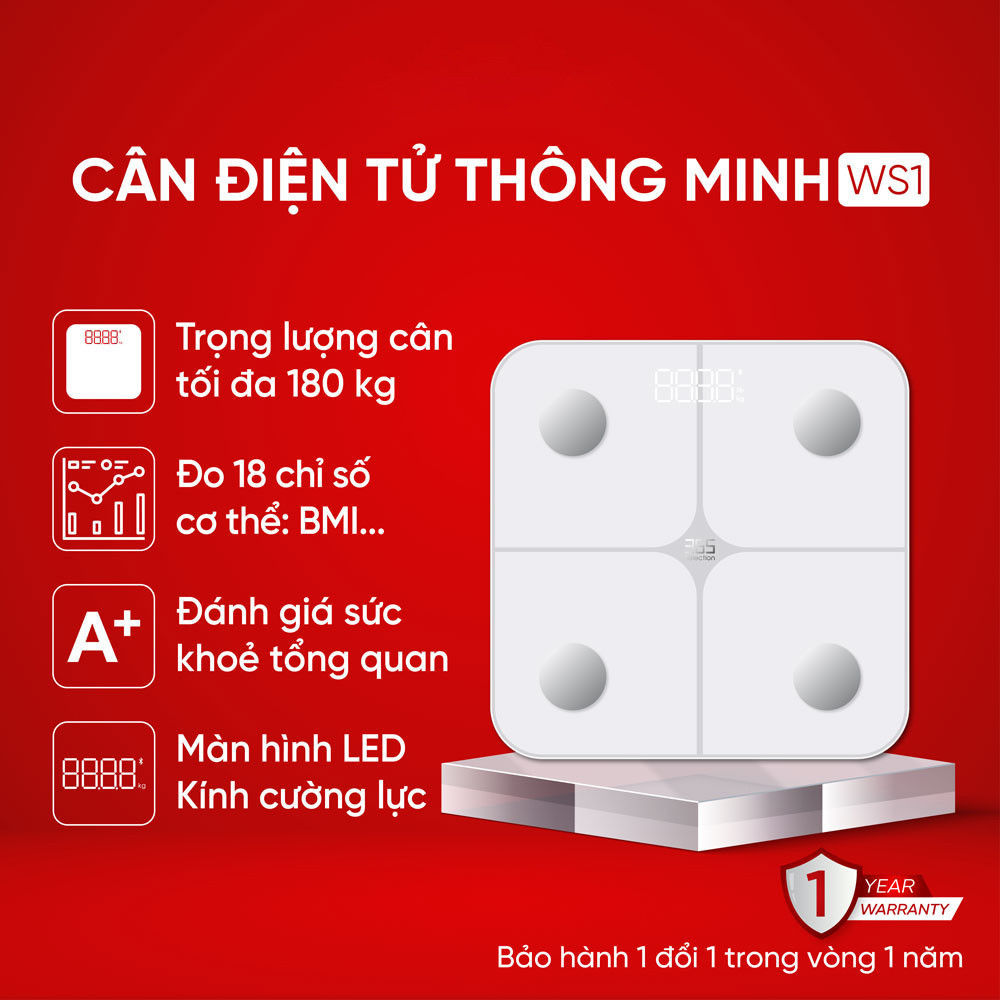
\includegraphics[width=0.6\linewidth]{graphics/ws1.png}
    \caption{Cân thông minh 365 Selection WS1}
\end{figure}

Được trang bị cảm biến chất lượng cao, cân thông minh 365 Selection WS1 đảm bảo đo lường trọng lượng với độ chính xác cao cùng tốc độ nhanh. Các cảm biến này cung cấp những thông số trọng lượng vô cùng chính xác và đáng tin cậy, cho phép người dùng đo lường và theo dõi trọng lượng cơ thể dễ dàng.

\begin{figure}[!htp]
    \centering
    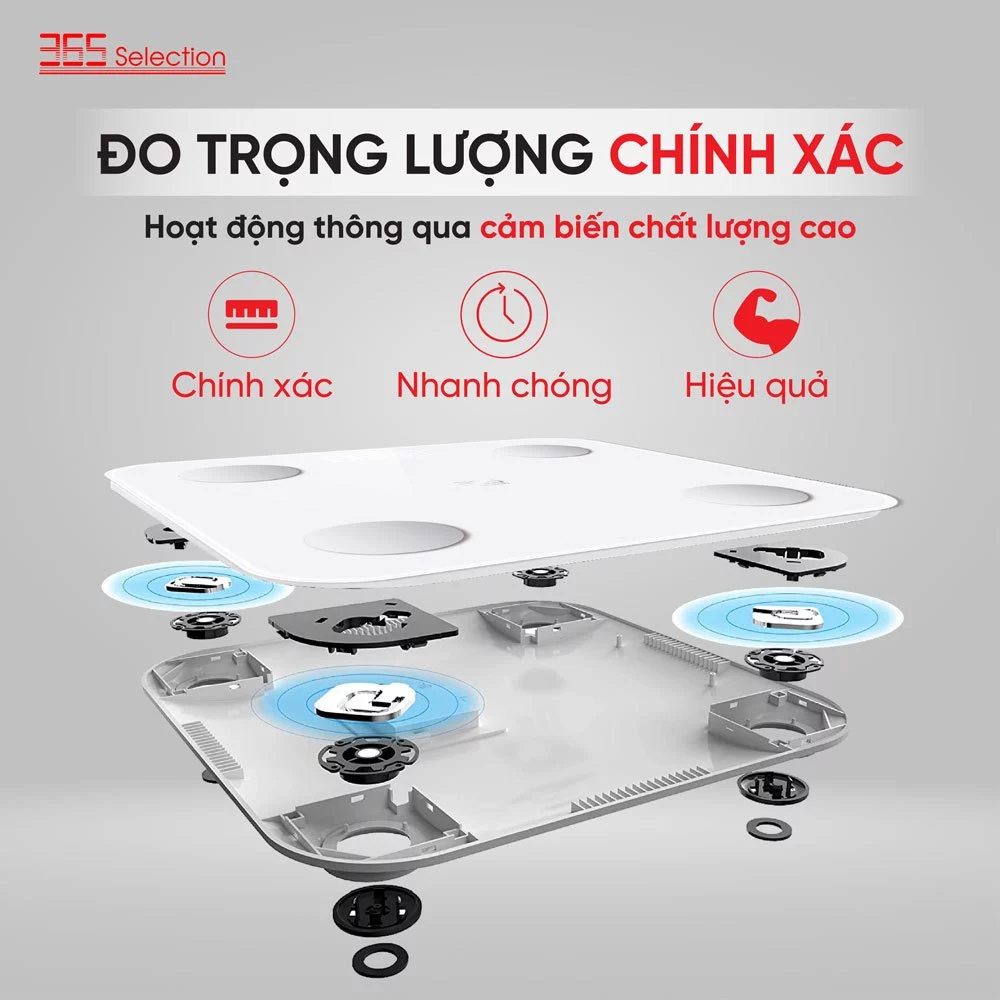
\includegraphics[width=0.6\linewidth]{graphics/sensors.png}
    \caption{Cảm biến chất lượng cao của WS1}
\end{figure}

Không chỉ đo trọng lượng chuẩn xác mà cân thông minh 365 Selection WS1 còn phân tích 18 chỉ số sức khoẻ quan trọng.

\begin{itemize}
    \item \textbf{Cân nặng:} Đo trọng lượng cơ thể tổng quát.
    \item BMI (Chỉ số khối cơ thể): Đánh giá sự cân đối giữa trọng lượng và chiều cao, giúp xác định mức độ béo phì hoặc thiếu cân.
    \item \textbf{Tỷ lệ mỡ cơ thể:} Xác định phần trăm mỡ so với tổng trọng lượng cơ thể, phản ánh mức độ mỡ cơ thể tổng quát.
    \item \textbf{Khối lượng cơ:} Đo lượng cơ bắp trong cơ thể, hữu ích để theo dõi sự phát triển cơ bắp và sức mạnh.
    \item \textbf{Khối lượng mỡ:} Đo lượng mỡ cơ thể toàn thân, giúp xác định mức độ mỡ dư thừa.
    \item \textbf{Chỉ số mỡ cơ thể:} Đánh giá mức độ phân bổ mỡ trong cơ thể, cung cấp cái nhìn về sự phân bố mỡ giữa các vùng cơ thể.
    \item \textbf{Mức độ béo phì:} Phân loại mức độ béo phì dựa trên tỷ lệ mỡ cơ thể và BMI, giúp xác định nguy cơ sức khỏe liên quan đến béo phì.
    \item \textbf{Cân nặng lý tưởng:} Cung cấp trọng lượng cơ thể lý tưởng dựa trên các yếu tố như chiều cao, tuổi, và giới tính.
    \item \textbf{Kiểm soát cân nặng:} Theo dõi sự thay đổi cân nặng theo thời gian để giúp bạn duy trì hoặc điều chỉnh mục tiêu cân nặng.
    \item \textbf{Chỉ số mỡ nội tạng:} Đo lượng mỡ xung quanh các cơ quan nội tạng, giúp đánh giá nguy cơ mắc bệnh tim mạch và các vấn đề sức khỏe khác.
    \item \textbf{Cân nặng trừ mỡ:} Xác định trọng lượng cơ thể sau khi trừ đi lượng mỡ, giúp phân tích khối lượng cơ và xương.
    \item \textbf{Nước trong cơ thể:} Đo lượng nước chiếm tỷ lệ trong cơ thể, phản ánh tình trạng hydrat hóa và sức khỏe tổng quát.
    \item \textbf{Khối lượng xương:} Đo lượng xương trong cơ thể, giúp theo dõi sức khỏe xương và nguy cơ loãng xương.
    \item \textbf{Tỷ lệ Protein:} Xác định tỷ lệ protein trong cơ thể, phản ánh tình trạng dinh dưỡng và sức khỏe cơ bắp.
    \item \textbf{BMR (Tỷ lệ trao đổi chất cơ bản):} Đánh giá số lượng calo cơ thể cần tiêu thụ để duy trì các chức năng cơ bản khi nghỉ ngơi.
    \item \textbf{Tuổi chuyển hóa:} Đo lường sự chuyển hóa cơ thể so với tuổi thực tế, giúp đánh giá tốc độ trao đổi chất và sức khỏe tổng quát.
    \item \textbf{Phân loại sức khỏe:} Xếp loại sức khỏe tổng thể dựa trên các chỉ số đo được, giúp bạn dễ dàng đánh giá tình trạng cơ thể.
    \item \textbf{Điểm số cơ thể:} Cung cấp một điểm số tổng hợp phản ánh tình trạng sức khỏe tổng thể, hỗ trợ bạn trong việc theo dõi và cải thiện lối sống.
\end{itemize}

Cân thông minh 365 Selection WS1 cho phép lưu trữ và cập nhật dữ liệu sức khoẻ trên ứng dụng 365 Life thông qua kết nối bluetooth. Cho phép người dùng nhanh chóng nắm bắt và theo dõi được tình trạng sức khoẻ qua từng lượt đo, có cái nhìn tổng quan về mức độ phát triển và tình trạng sức khoẻ của người dùng.

\newpage

\begin{figure}[!htp]
    \centering
    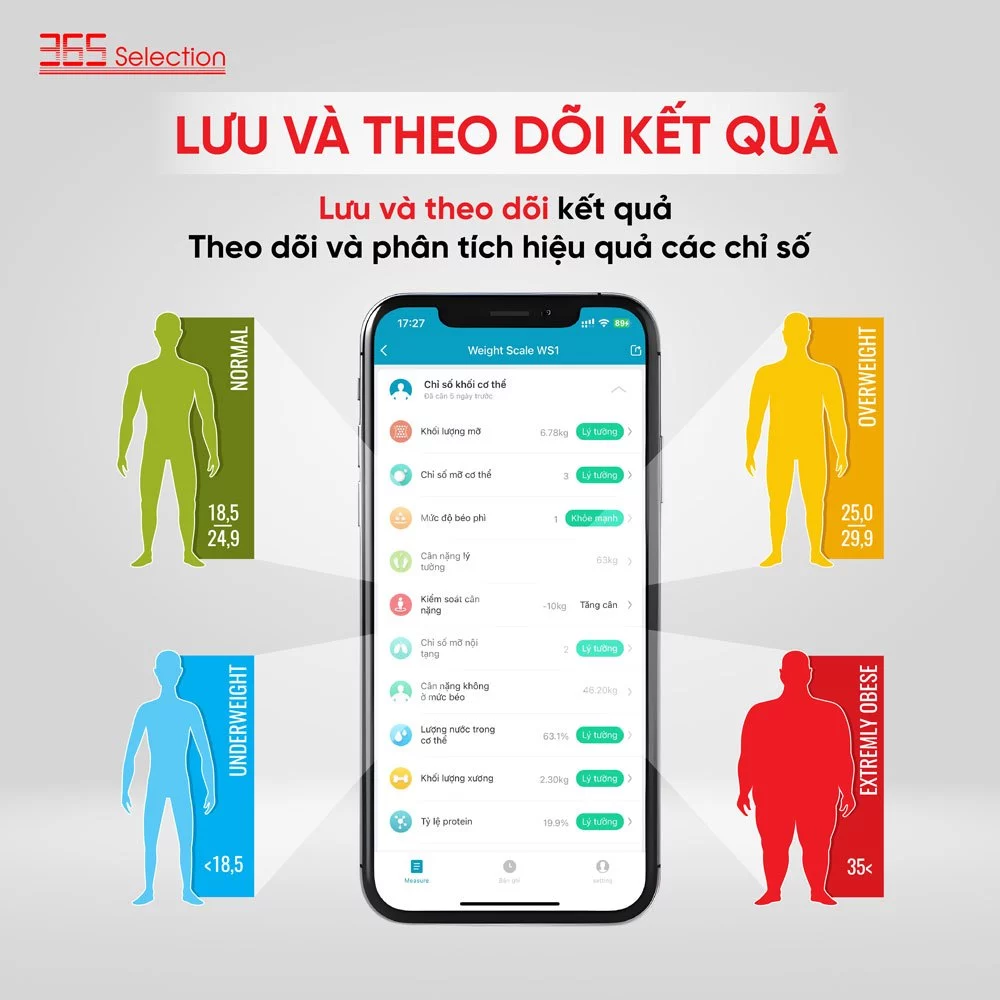
\includegraphics[width=0.6\linewidth]{graphics/theodoichiso.png}
    \caption{Khả năng lưu trữ và cập nhật dữ liệu}
\end{figure}

Ngoài ra, sản phẩm còn hỗ trợ lưu trữ kết quả đo cho tối đa 10 người, cân thông minh sẽ cho phép tất cả gia đình cùng sử dụng. Cân sẽ tự động nhận diện người sử dụng dựa trên các dữ liệu trước đó hoặc nhận diện người mới khi các chỉ số được đo. Trong ứng dụng 365 Life, kết quả đo sẽ được lưu trữ tự động, giúp bạn giám sát và theo dõi tình hình sức khoẻ của các thành viên trong gia đình một cách thuận tiện và dễ dàng.

\subsection{Thách thức và cơ hội triển khai tại Việt Nam}

Việt Nam đang trong giai đoạn thúc đẩy mạnh mẽ quá trình chuyển đổi số trong nhiều lĩnh vực, bao gồm cả y tế. Các cơ hội để phát triển và triển khai hệ thống chăm sóc sức khỏe điện tử rất lớn, nhờ vào sự hỗ trợ từ chính sách của chính phủ và tốc độ phát triển công nghệ. Cùng với sự phát triển của hạ tầng viễn thông và Internet, người dân Việt Nam ngày càng có khả năng tiếp cận các dịch vụ y tế thông minh, từ đó giúp nâng cao ý thức về chăm sóc sức khỏe.

Tuy nhiên, việc triển khai hệ thống chăm sóc sức khỏe điện tử tại Việt Nam vẫn đối mặt với một số thách thức. Đầu tiên là vấn đề về hạ tầng công nghệ, đặc biệt ở các khu vực nông thôn và vùng sâu, vùng xa. Khả năng tiếp cận Internet và các thiết bị thông minh ở những khu vực này còn hạn chế, do đó việc triển khai hệ thống có thể gặp khó khăn trong việc tiếp cận người dùng. Thứ hai, là vấn đề bảo mật và quyền riêng tư của dữ liệu sức khỏe cá nhân. Khi dữ liệu sức khỏe được thu thập và lưu trữ trên các hệ thống đám mây, cần có các biện pháp bảo mật chặt chẽ để đảm bảo không xảy ra các sự cố lộ lọt thông tin cá nhân.

\subsection{Tầm quan trọng của hệ thống trong tương lai}

Việc xây dựng một hệ thống chăm sóc sức khỏe điện tử với thiết bị CRENOT Gofit S2 phù hợp với xu hướng toàn cầu về chăm sóc sức khỏe thông minh, đồng thời góp phần vào việc cải thiện chất lượng chăm sóc sức khỏe tại Việt Nam. Hệ thống không chỉ đáp ứng nhu cầu của cá nhân trong việc theo dõi sức khỏe mà còn cung cấp một công cụ hỗ trợ đắc lực cho các cơ sở y tế trong quản lý sức khỏe cộng đồng, giảm tải gánh nặng cho hệ thống y tế hiện tại.

Với sự phát triển của trí tuệ nhân tạo và phân tích dữ liệu lớn, tương lai của hệ thống chăm sóc sức khỏe điện tử sẽ càng trở nên thông minh và hiệu quả hơn. Các công nghệ này sẽ giúp cá nhân hóa các giải pháp chăm sóc sức khỏe, từ đó không chỉ tăng cường chất lượng cuộc sống của người dân mà còn góp phần vào sự phát triển bền vững của hệ thống y tế Việt Nam.